%
% gauss.tex
%
% (c) 2021 Prof Dr Andreas Müller, Hochschule Rapperswil
%
\bgroup
\def\ds{0.5}
\def\punkt#1#2{({(#1)*\ds},{-(#2)*\ds})}
\def\tabelle{
	\foreach \x in {-0.5,0.5,3.5}{
		\draw \punkt{\x}{-0.5} -- \punkt{\x}{3.5};
		\draw \punkt{-0.5}{\x} -- \punkt{3.5}{\x};
	}
	\node at \punkt{0}{1} {$0$};
	\node at \punkt{0}{2} {$1$};
	\node at \punkt{0}{3} {$2$};
	\node at \punkt{1}{0} {$0$};
	\node at \punkt{2}{0} {$1$};
	\node at \punkt{3}{0} {$2$};
}
\begin{frame}[t]
\frametitle{Gauss-Algorithmus in $\mathbb{F}_3$}
\setlength{\abovedisplayskip}{5pt}
\setlength{\belowdisplayskip}{5pt}
\begin{columns}[t,onlytextwidth]
\begin{column}{0.44\textwidth}
\begin{block}{Additions-/Multiplikationstabelle}
\begin{center}
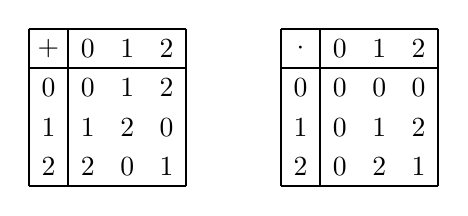
\begin{tikzpicture}[>=latex,thick]
\begin{scope}[xshift=-1.6cm]
\tabelle
\node at \punkt{0}{0} {$+$};
\node at \punkt{1}{1} {$0$};
\node at \punkt{1}{2} {$1$};
\node at \punkt{1}{3} {$2$};
\node at \punkt{2}{1} {$1$};
\node at \punkt{2}{2} {$2$};
\node at \punkt{2}{3} {$0$};
\node at \punkt{3}{1} {$2$};
\node at \punkt{3}{2} {$0$};
\node at \punkt{3}{3} {$1$};
\end{scope}
\begin{scope}[xshift=1.6cm]
\tabelle
\node at \punkt{0}{0} {$\cdot$};
\node at \punkt{1}{1} {$0$};
\node at \punkt{1}{2} {$0$};
\node at \punkt{1}{3} {$0$};
\node at \punkt{2}{1} {$0$};
\node at \punkt{2}{2} {$1$};
\node at \punkt{2}{3} {$2$};
\node at \punkt{3}{1} {$0$};
\node at \punkt{3}{2} {$2$};
\node at \punkt{3}{3} {$1$};
\end{scope}
\end{tikzpicture}
\end{center}

\end{block}
\end{column}
\begin{column}{0.52\textwidth}
\uncover<2->{%
\begin{block}{Gleichungssystem\uncover<9->{/Lösung}}
\[
\left.
\begin{array}{rcrcrcrcr}
 x&+&y&+2z&=&1\\
2x& & &+ z&=&2\\
 x&+&y&   &=&2
\end{array}
\uncover<9->{
\right\}
\Rightarrow
\left\{
\begin{aligned}
x&=2\\
y&=0\\
z&=1
\end{aligned}
\right.}
\]
\end{block}}
\end{column}
\end{columns}
\uncover<3->{%
\begin{block}{Gauss-Algorithmus}
\begin{center}
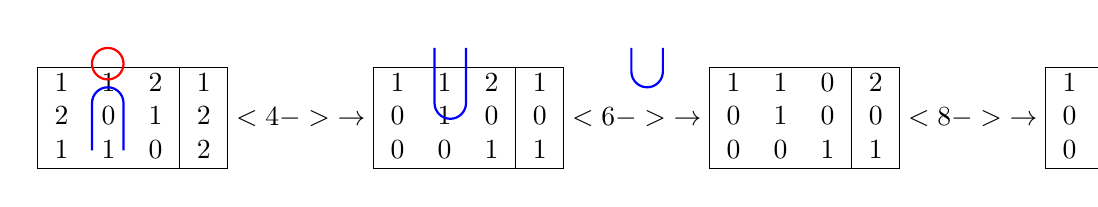
\begin{tikzpicture}[>=latex,thick]
\node at (0,0) {\begin{minipage}{13cm}%
\[
\begin{tabular}{|>{$}c<{$}>{$}c<{$}>{$}c<{$}|>{$}c<{$}|}
\hline
 1 & 1 & 2 & 1 \\
 2 & 0 & 1 & 2 \\
 1 & 1 & 0 & 2 \\
\hline
\end{tabular}
\uncover<4->{%
\to
\begin{tabular}{|>{$}c<{$}>{$}c<{$}>{$}c<{$}|>{$}c<{$}|}
\hline
 1 & 1 & 2 & 1 \\
 0 & 1 & 0 & 0 \\
 0 & 0 & 1 & 1 \\
\hline
\end{tabular}}
\uncover<6->{%
\to
\begin{tabular}{|>{$}c<{$}>{$}c<{$}>{$}c<{$}|>{$}c<{$}|}
\hline
 1 & 1 & 0 & 2 \\
 0 & 1 & 0 & 0 \\
 0 & 0 & 1 & 1 \\
\hline
\end{tabular}}
\uncover<8->{%
\to
\begin{tabular}{|>{$}c<{$}>{$}c<{$}>{$}c<{$}|>{$}c<{$}|}
\hline
 1 & 0 & 0 & 2 \\
 0 & 1 & 0 & 0 \\
 0 & 0 & 1 & 1 \\
\hline
\end{tabular}}
\]
\end{minipage}};
\begin{scope}[yshift=0.2cm]
\uncover<3->{
\draw[color=red] (-5.6,0.3) circle[radius=0.2];
\draw[color=blue] (-5.4,-0.8) -- (-5.4,-0.2) arc (0:180:0.2) -- (-5.8,-0.8);
}
\uncover<5->{
\draw[color=blue] (-1.45,0.5) -- (-1.45,-0.2) arc (180:360:0.2) -- (-1.05,0.5);
}
\uncover<7->{
\draw[color=blue] (1.05,0.5) -- (1.05,0.2) arc (180:360:0.2) -- (1.45,0.5);
}
\end{scope}
\end{tikzpicture}
\end{center}
\end{block}}
\end{frame}
\egroup
